\chapter{Guaranteed Escape Speed}
\label{chap:nonconservative}
\graphicspath{{Results/Images/}}

In this chapter, we will discuss the results from the \gls{NCGES} analytical method developed in \Cref{sec:escape_speed_derivation}. The algorithm's absolute performance and its viability is discussed and compared with that of the \gls{CGES} algorithm. Note that the results in this chapter were obtained for simulations conducted without adding Solar perturbations.

\section{Simulation Setup}
\label{sec:nonconservative_simulation_setup}
As mentioned in \Cref{sec:escape_speed_derivation}, the launch location for testing out the algorithm was chosen to be the longest edge of the ellipsoid shaped asteroid since it helped in simplifying the computations. In addition to this, the particles were launched in the equatorial plane such that the orbital inclination remained zero \footnote{The orbital inclination remains zero valued after the launch in a non-uniform gravity field because the central body is homogeneous as well as symmetrical about the equator which means that there is equal attraction in the positive and negative z-axis directions, which cancel each other out.}, which further simplified the computation.
%
\newline\newline
%
We compare the results from our derivation of the \gls{NCGES} algorithm, with that of the conservative approach as defined by \cite{scheeresBook}. To do the comparison, the following launch conditions were used (these launch conditions are also depicted in \Cref{fig:non_conservative_launch_vectors} for a few launch declination angles):
%%%
\begin{enumerate}
    \item The launch location is at the longest edge of the ellipsoid.
    \item The launch azimuth is equal to \SI{270}{\degree}.
    \item The launch declinations are varied from \SI{10}{\degree} to \SI{80}{\degree}.
    \item The launch velocity was kept fixed and chosen at random to be \SI{6.0}{\metre \per \second}.
\end{enumerate}
%%%
Note that these launch conditions result in equatorial orbits, just like how we want, to test the \gls{NCGES} algorithm. The value for the parameter $q_\infty$ in \Cref{eqn:non_conservative_inertial_guaranteed_escape_speed}, which is the periapsis distance for a parabolic escape trajectory, was set manually for each simulated trajectory and remained constant during the entire duration of each simulation. Several values of $q_\infty$ were used for testing and they were all taken as fractions of the largest dimension of the ellipsoid. This was done because we do not yet have a dedicated process to determine the value of $q_\infty$ and hence several random fractions were used to gauge the output.
% Note that $q_\infty$ is the distance from the focus to the vertex of a parabola so in this case it is the distance between the centre of the asteroid and the periapsis distance on the final parabolic escape trajectory. We say \emph{final} because the \gls{NCGES} was designed to account for regolith cases that do not immediately lead to an escape scenario after being lofted from the surface of an asteroid but rather take one or more orbital revolutions around the asteroid before embarking on the parabolic escape trajectory. We will witness such a case shortly.
% %
% \newline\newline
% %
% To highlight the effectiveness of the \gls{CGES} method with a uniform gravity field, we conduct simulations for particles lofted from an equatorial site on a spherical asteroid of radius \SI{10}{\kilo\metre}. The initial conditions for this simulation are stated as follows:
% %%%
% \begin{enumerate}
%     \item The launch location is on the equator of the spherical asteroid.
%     \item Launch azimuths are varied from \SI{0}{\degree} to \SI{360}{\degree}.
%     \item The launch declination is kept constant at \SI{45}{\degree}.
%     \item Launch velocities are varied from 1 to \SI{20}{\metre\per\second}.
% \end{enumerate}
%%%
%%%
\begin{figure}[htb]
\centering
\captionsetup{justification=centering}
\subfloat[]{
    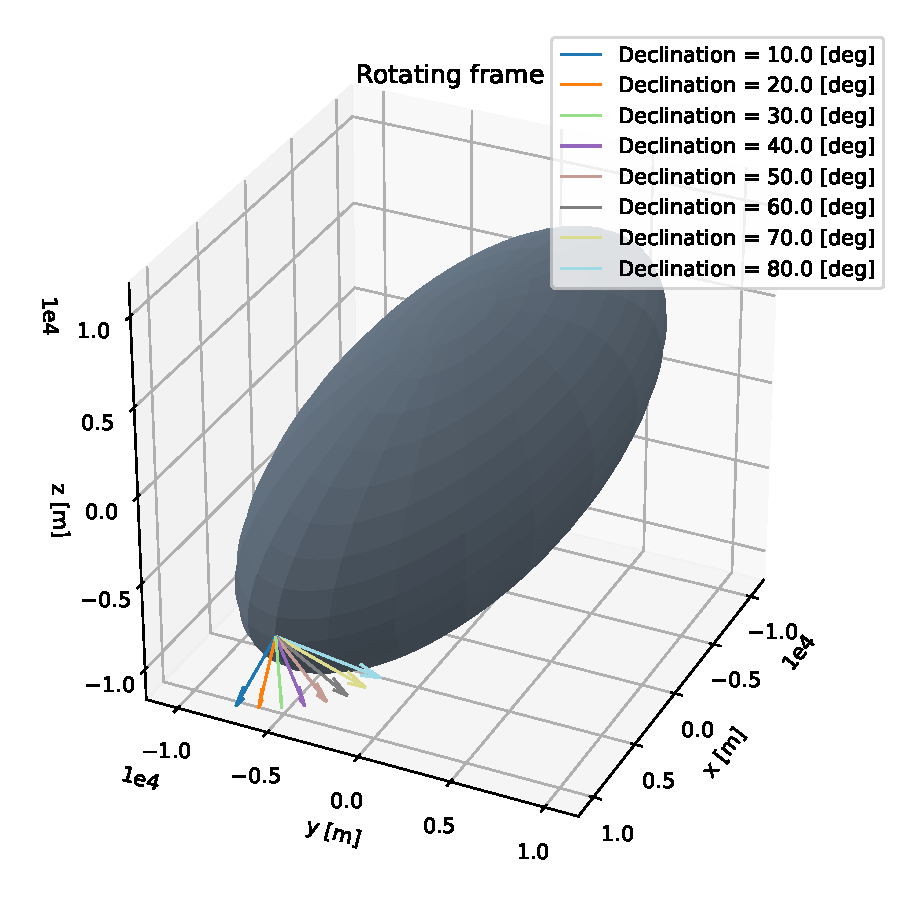
\includegraphics[width=0.4\textwidth, height=0.5\textheight, keepaspectratio=true]{non_conservative_escape_speed/launch_vectors_body_frame.pdf}
    \label{fig:non_conservative_launch_vectors_arf}
}
\subfloat[]{
    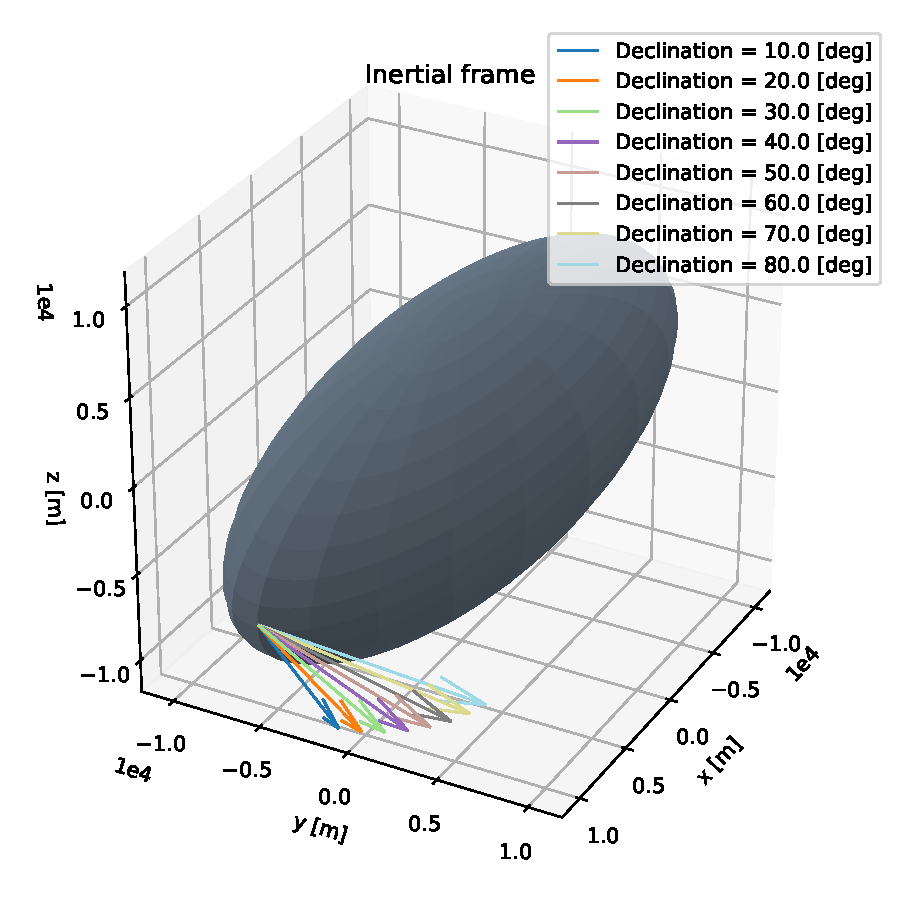
\includegraphics[width=0.4\textwidth, height=0.5\textheight, keepaspectratio=true]{non_conservative_escape_speed/launch_vectors_inertial_frame.pdf}
    \label{fig:non_conservative_launch_vectors_aif}
}
\caption{Launch vectors used for testing the \gls{NCGES} algorithm. \protect\subref{fig:non_conservative_launch_vectors_arf} Vectors expressed in the \gls{ARF} and \protect\subref{fig:non_conservative_launch_vectors_aif} Vectors expressed in the \gls{AIF}.}
\label{fig:non_conservative_launch_vectors}
\end{figure}
\FloatBarrier
%%%
%%%
\begin{figure}[htb]
\centering
\captionsetup{justification=centering}
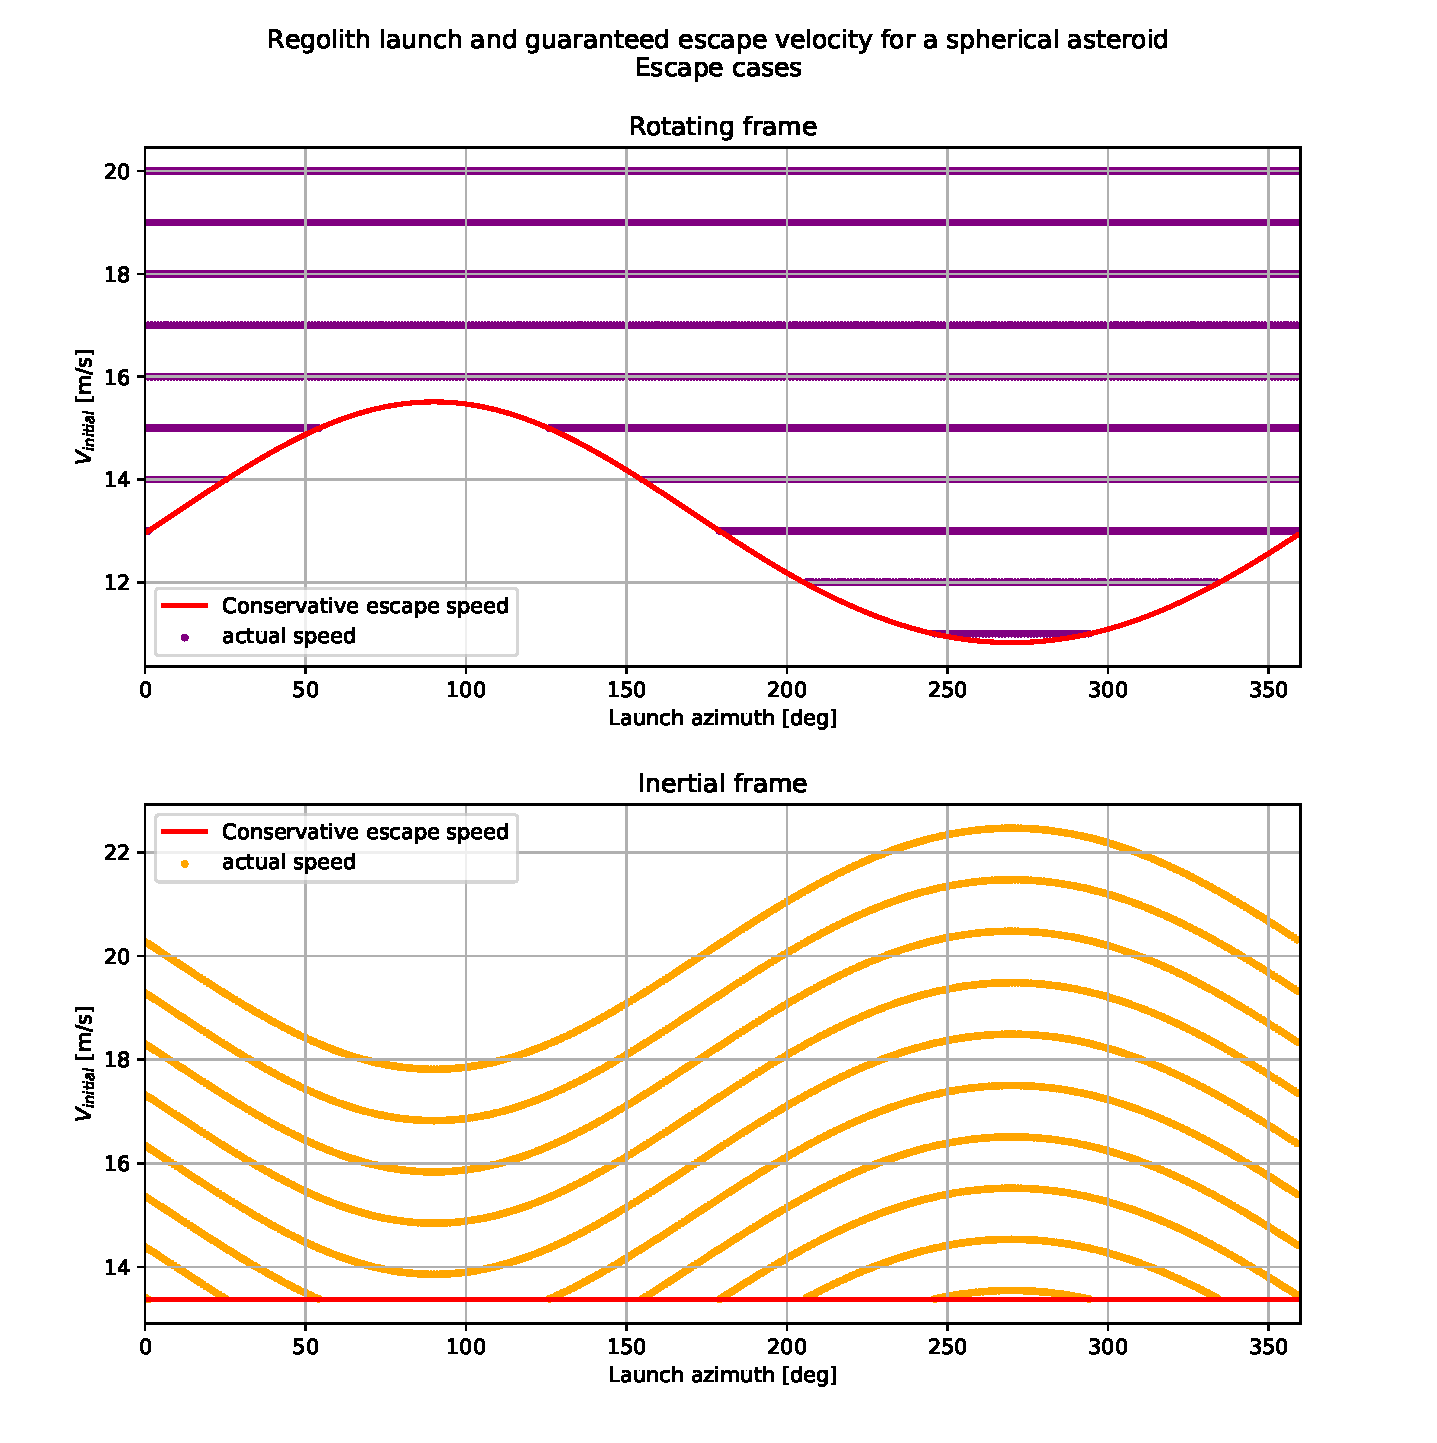
\includegraphics[width=\textwidth, height=0.5\textheight, keepaspectratio=true]{non_conservative_escape_speed/spherical_asteroid_conservative_escape_speed.pdf}
\caption{Escape velocities for varying launch azimuths and a constant launch declination of \protect\SI{45}{\degree}. The \gls{CGES} curve clearly separates all escape scenarios, as shown in both the \protect\gls{AIF} and the \protect\gls{ARF}. Note that for the launch azimuth of \SI{270}{\degree}, the \gls{CGES} is lower than that for the launch azimuth of \SI{90}{\degree}. This is because in case of the former, the particle is launched in the direction of rotation of the asteroid, whereas in case of the latter, the particle is launched against the rotational direction.}
\label{fig:conservative_spherical_asteroid_escape}
\end{figure}
\FloatBarrier
%%%
\section{Conservative Approach With Spherical Asteroid}
\label{sec:conservative_spherical_asteroid_results}
We will first look at the case of a homogeneous spherical asteroid whose radius is equal to \SI{10}{\kilo\metre}. The simulation involved launching particles at a constant declination of \SI{45}{\degree} and for launch azimuth varying in the range [0, 360)\si{\degree}. The launch velocities ranged from 1 - \SI{20}{\metre \per \second} and the simulations did not include perturbations, gravity or otherwise. We used the \gls{CDE} potential model but all three semi-axes were made equal to \SI{10}{\kilo\metre}. In such a case, the \gls{CDE} gravity potential model acts like a point mass potential model. This situation works for us since the latter is the actual gravity potential model for a point external to a homogeneous spherical body \parencite{macmillanPotential}.
%
\newline\newline
%
The algorithm for the \gls{CGES} works properly for the case of a homogeneous spherical asteroid, as shown in \Cref{fig:conservative_spherical_asteroid_escape}, whose gravity potential is equivalent to that of a point mass. An escape occurs only if the particle was launched with a velocity which is equal to or above the \gls{CGES} curve and not otherwise. \Cref{fig:conservative_spherical_asteroid_escape_and_reimpact} shows how the curve even separates out all the re-impact cases. All launch velocities that are below the escape speed curve result only in re-impact and nothing else. Note that for this particular simulation we did not obtain any capture cases, but only escape and re-impact.
%%%
\begin{figure}[htb]
\centering
\captionsetup{justification=centering}
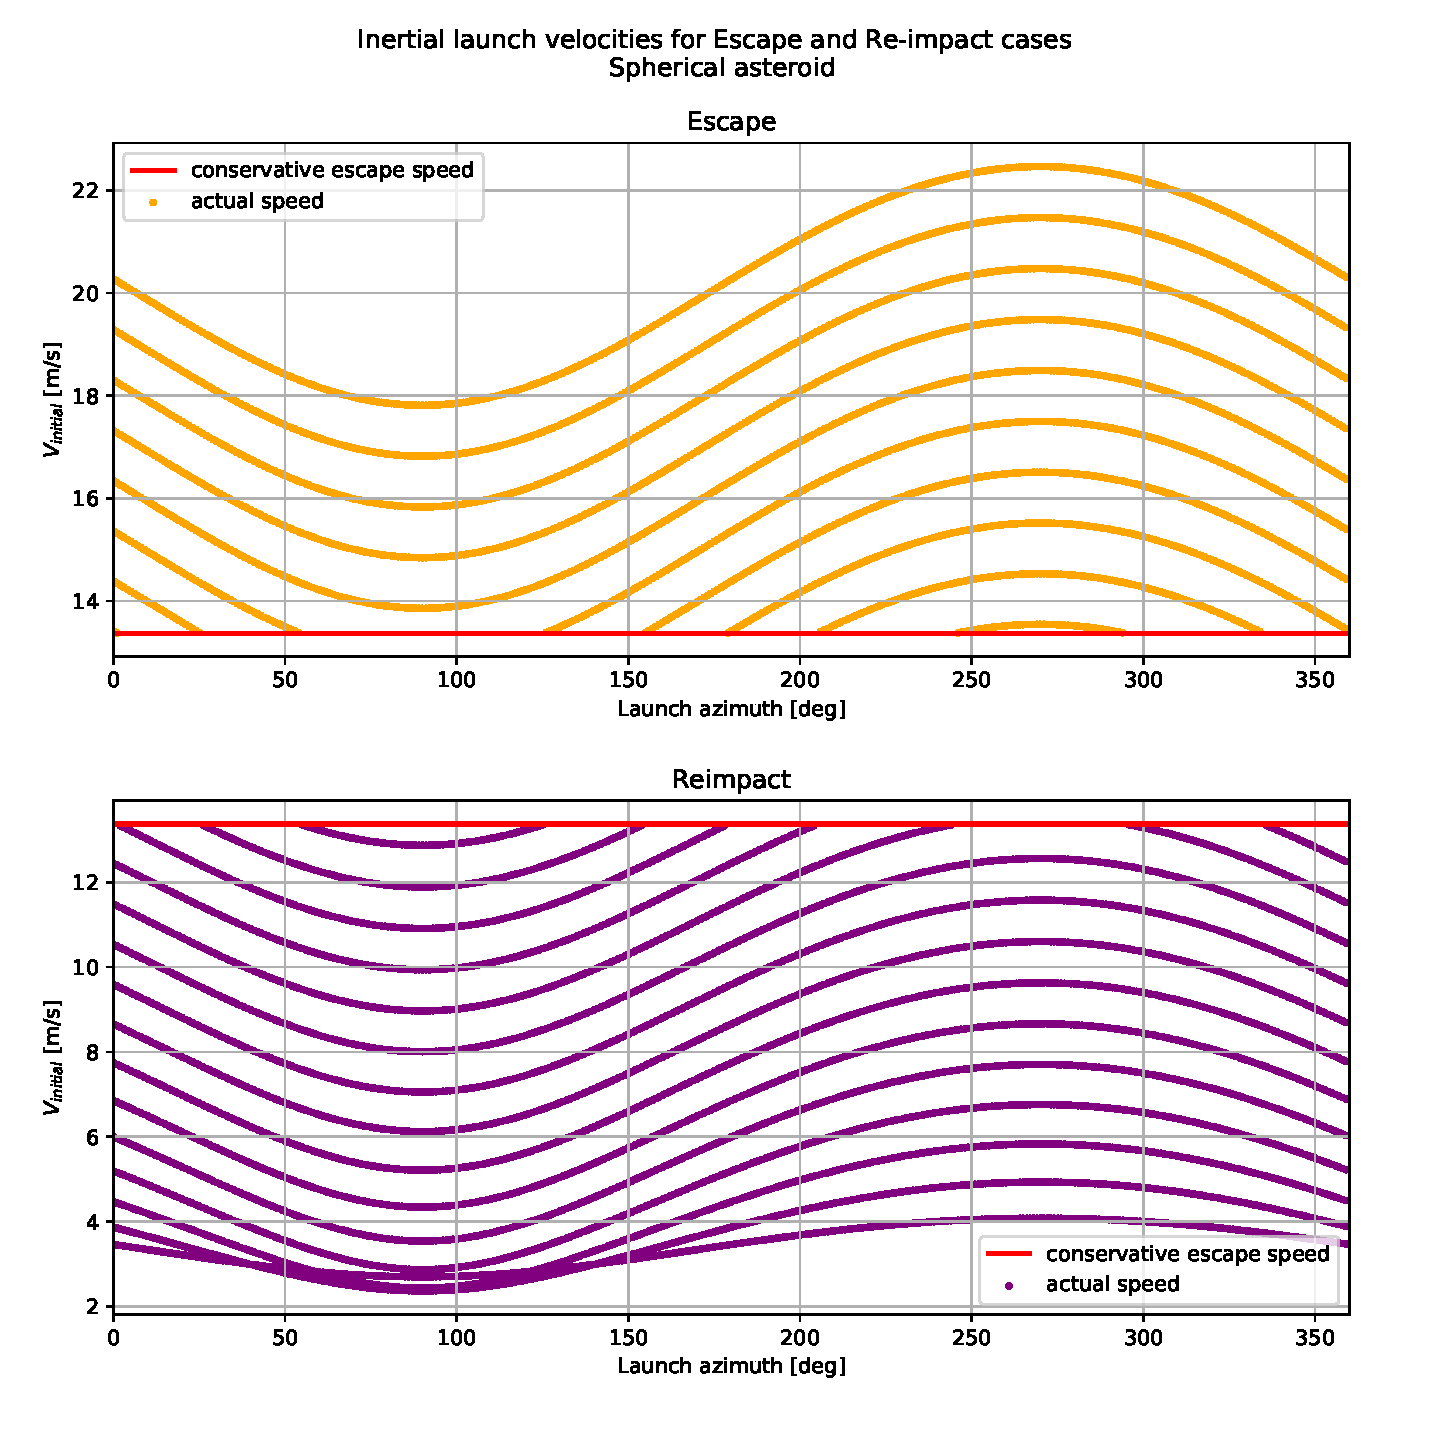
\includegraphics[width=\textwidth, height=0.5\textheight, keepaspectratio=true]{non_conservative_escape_speed/spherical_asteroid_escape_and_capture.pdf}
\caption{Escape and re-impact scenario velocities for varying launch azimuths and a constant launch declination of \protect\SI{45}{\degree}. The \gls{CGES} curve clearly separates all re-impact cases from the escape ones.}
\label{fig:conservative_spherical_asteroid_escape_and_reimpact}
\end{figure}
\FloatBarrier
%%%
\section{Non-Conservative Approach With Ellipsoidal Asteroid}
\label{sec:nonconservative_escape_cde_results}
Now we shall look at the results for the \gls{CDE} model, for which particles were launched with the initial conditions enlisted in \Cref{sec:nonconservative_simulation_setup}. Before we can analyze the result in \Cref{fig:non_conservative_escape_multiple_qinfinity_single_velocity}, it is important to discuss its structure. In the figure, the pink and the green region in the background depict the final fate regime associated with the varying launch declination angles and the singular launch velocity of \SI{6}{\metre\per\second}. The white spaces in the background of the plot have no meaning; they are there because of the transition in the final fate regime from one azimuth angle to the next one. Although the highlighted (pink or green) regions span the entire y-axis in \Cref{fig:non_conservative_escape_multiple_qinfinity_single_velocity}, they do not represent the final fate for any other velocity along that axis apart from the launch velocity of \SI{6}{\metre\per\second}. Hence, the highlighted regions are also not fixed for the given range of declination angles.
% The white spaces in between the pink and the green regions point out the cases which resulted in neither an escape nor a re-impact. These are also not capture cases as upon closer inspection, we saw that these cases have high altitude orbits with extremely high eccentricities such that the particles do not even complete a single revolution before the end of the simulation.
%
\newline\newline
%
\Cref{fig:non_conservative_escape_multiple_qinfinity_single_velocity} shows the inadequacy of the \gls{CGES} algorithm to predetermine escape scenarios based just on the initial conditions, as it fails to account for escape situations that occur at lower declination angles. In this particular situation, the particles are being lofted with a single value for the launch velocity i.e. \SI{6}{\metre\per\second} (depicted by the purple line in \Cref{fig:non_conservative_escape_multiple_qinfinity_single_velocity}) and whenever this value is above the \gls{CGES} curve (depicted by the black line in \Cref{fig:non_conservative_escape_multiple_qinfinity_single_velocity}), we see that the particle always escapes. Note that its not necessary for particles to escape when their launch velocity is above the \gls{CGES}, especially when they are not launched in the normal direction; a discussion on this is presented later in \Cref{sec:conservative_escape_cde_limitations}. The \gls{NCGES} algorithm, however, does not function as expected. The algorithm was designed, hoping that it would also account for escape cases that the conservative approach was unable to. \Cref{fig:non_conservative_escape_multiple_qinfinity_single_velocity} shows the \gls{NCGES} curves for three different $q_\infty$ values. The algorithm fails to identify escape scenarios since there are cases at higher declination angles, where the launch velocity lies below the \gls{NCGES} curves, but the particle still escapes.
%%%
\begin{figure}[!h]
\centering
\captionsetup{justification=centering}
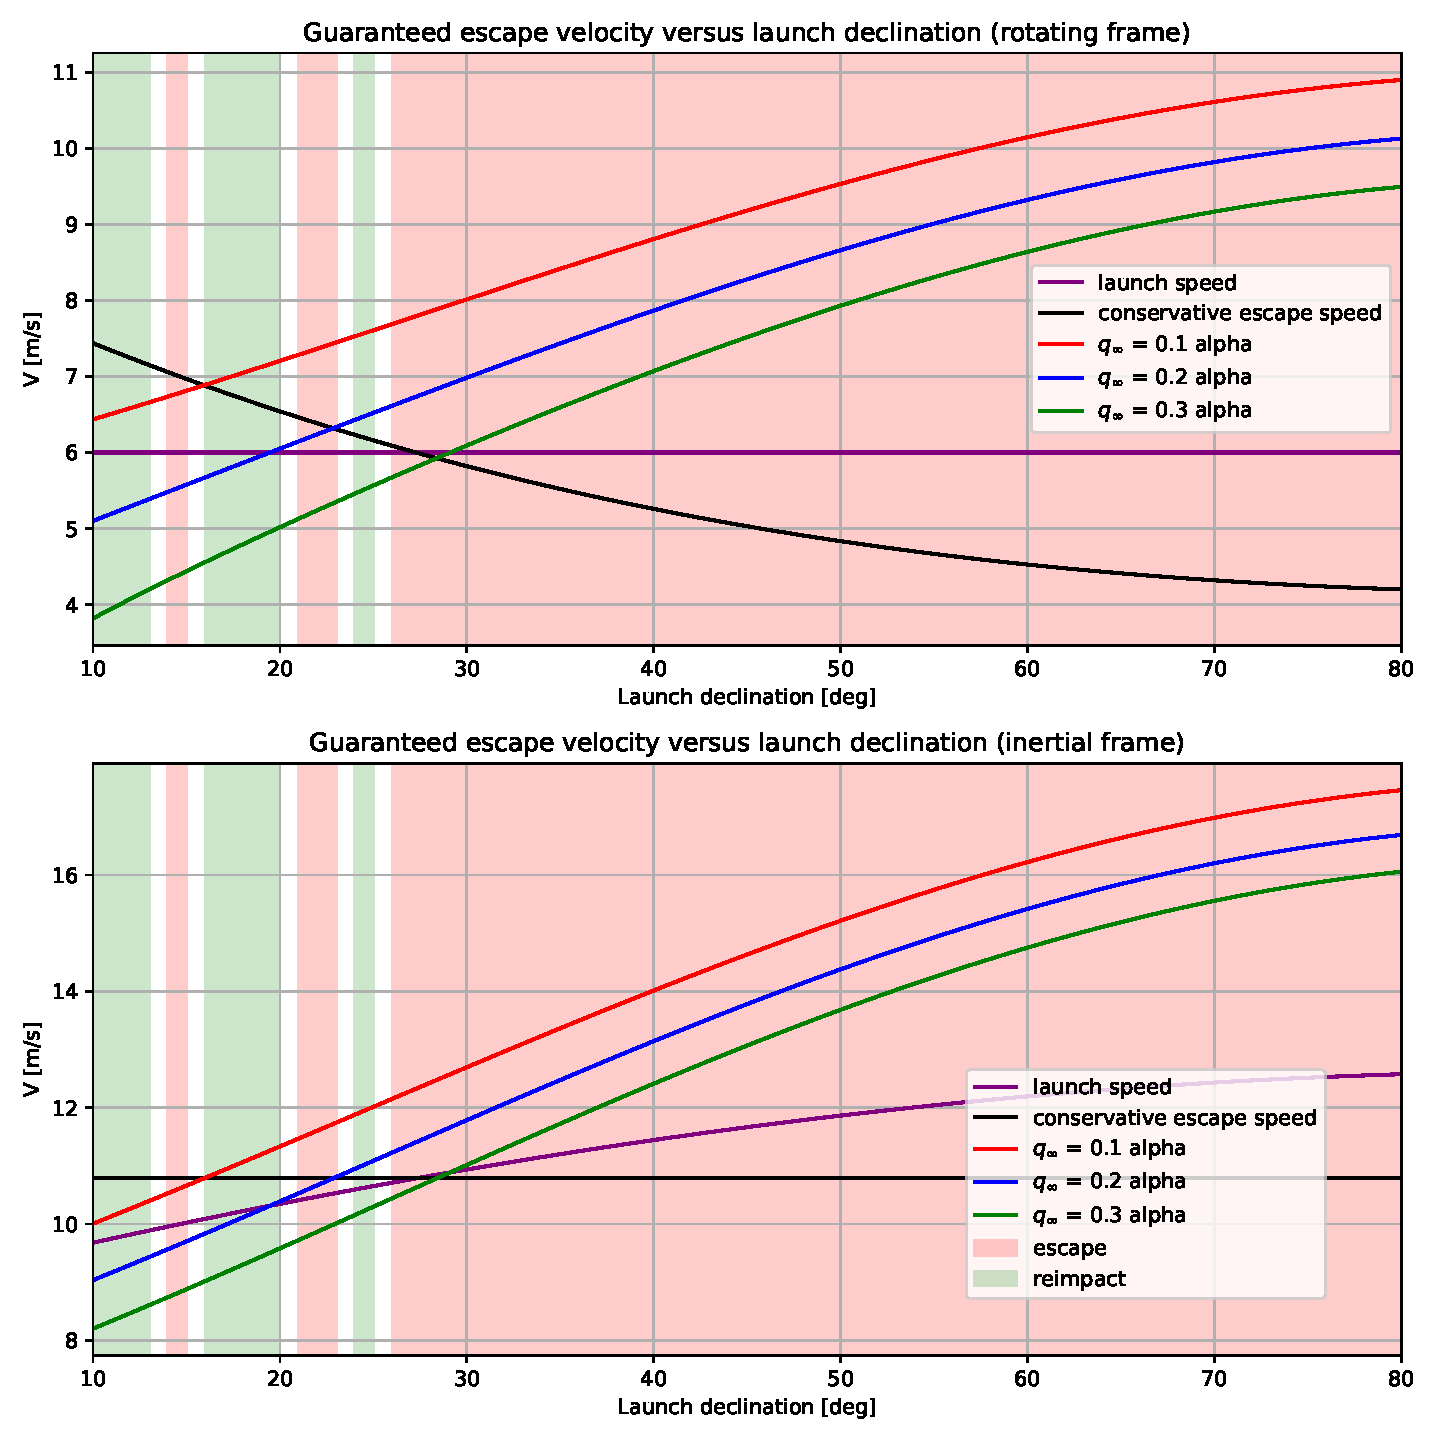
\includegraphics[width=\textwidth, height=0.5\textheight, keepaspectratio=true]{non_conservative_escape_speed/multiple_qinfinity_plus.pdf}
\caption{Escape and re-impact scenarios depicted for regolith launched with a single velocity and launch azimuth but multiple launch declination values. \gls{NCGES} curve is shown for a \gls{CDE} asteroid for three $q_\infty$ values that are fractions of the largest semi-axes, $\alpha$, of the ellipsoid. The \gls{CGES} curve is also shown for comparison.}
\label{fig:non_conservative_escape_multiple_qinfinity_single_velocity}
\end{figure}
\FloatBarrier
%%%
It is important to note that in \Cref{fig:non_conservative_escape_multiple_qinfinity_single_velocity}, the \gls{NCGES} curves used only the \emph{"+"} sign part of the formula in \Cref{eqn:non_conservative_inertial_guaranteed_escape_speed} and not the \emph{"-"} sign part since the latter always gave negative velocities for multiple sample values of $q_\infty$. We performed the simulation for the \gls{NCGES} approach for the same launch azimuth and range of declination angles as before but velocities ranging from 1 to \SI{16}{\metre\per\second} and $q_\infty=0.3$ to see if the curve provides better escape estimates at other launch velocities. The result of this is shown in \Cref{fig:non_conservative_multiple_velocities_qinfinity_0.3}. We see yet again the failure of the so called \gls{NCGES} algorithm. It is observed that even when the launch velocity is above the \gls{NCGES} curve, we have re-impact scenarios. This clearly means that the algorithm is not even able to demarcate re-impact situations. However, this situation is also true for the \gls{CGES} method as we see a few re-impact cases where the launch velocity is above the \gls{CGES} curve. Note that there is a limitation when it comes to the \gls{CGES} in demarcating all re-impact cases and this is discussed later in \Cref{sec:conservative_escape_cde_limitations}.
%%%
\begin{figure}[htb]
\centering
\captionsetup{justification=centering}
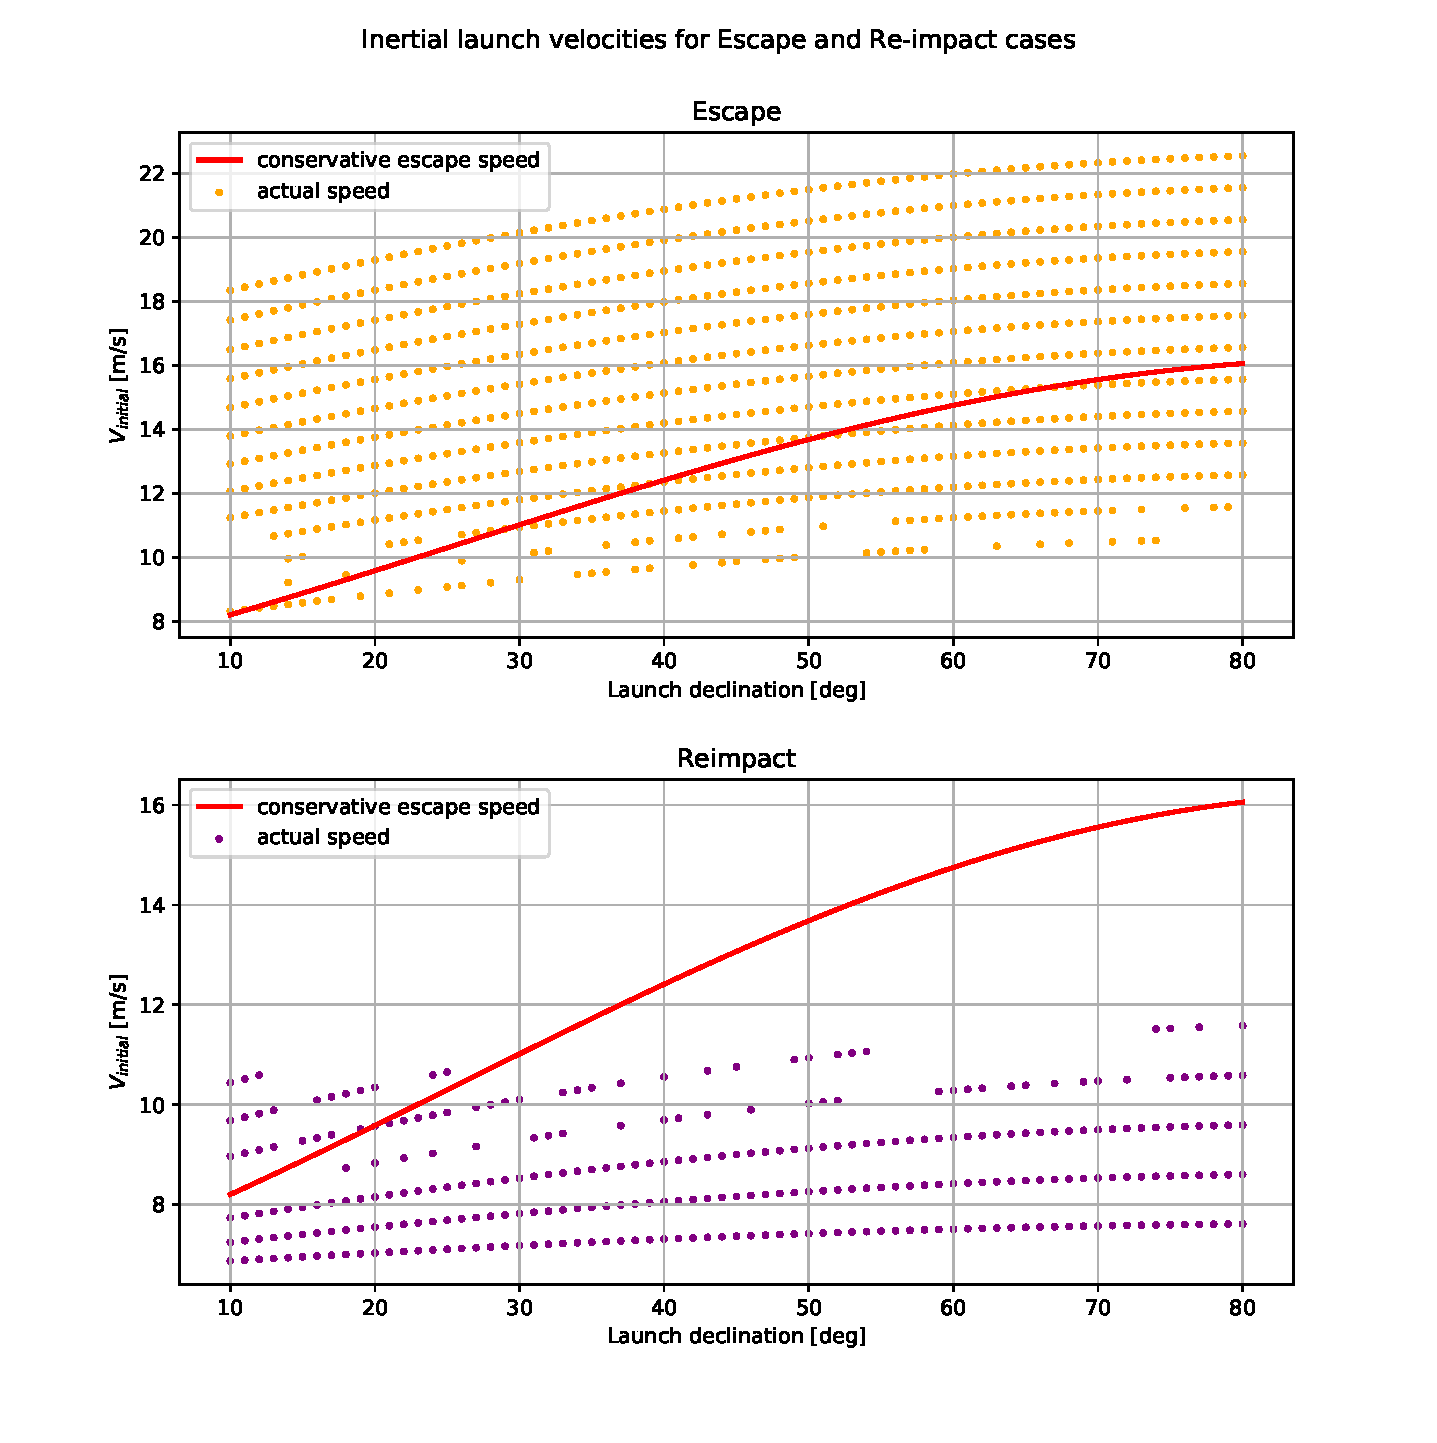
\includegraphics[width=\textwidth, height=0.5\textheight, keepaspectratio=true]{non_conservative_escape_speed/qinfinity_dot3_escape_reimpact_multipleVelocities_corrected.pdf}
\caption{Escape and re-impact scenarios depicted for regolith launched from the longest edge of \gls{CDE} with multiple velocities; with launch azimuth = \SI{270}{\degree} and launch declination in the range of \SI{10}{\degree} to \SI{80}{\degree}. The \gls{NCGES} curve is shown for $q_\infty = 0.3$.}
\label{fig:non_conservative_multiple_velocities_qinfinity_0.3}
\end{figure}
\FloatBarrier
%%%
On the other end of the spectrum, we can see that there are launch velocities below the \gls{NCGES} curve where escape scenarios occur. This is another indication of the failure of the algorithm we derived.
%
\newline\newline
%
Apart from the inability to completely differentiate between escape and re-impact cases, as we observed in \Cref{fig:non_conservative_multiple_velocities_qinfinity_0.3}, another problem with the \gls{NCGES} algorithm is that if we increase the value of $q_\infty$ beyond certain extent, then we obtain a meaningless curve for the \gls{NCGES} in the \gls{ARF}. An example of this is depicted in \Cref{fig:non_conservative_qinfinity_0.7} where $q_\infty = 0.7$. The curve as expressed in the \gls{ARF} has no meaning since negative speeds are not valid. Thus for a relatively high $q_\infty$ value, the output of \gls{NCGES} provides invalid values of speeds, thereby pointing to the failure of the method on two accounts. The \gls{NCGES} method did not work as expected in identifying the escape cases that were undetected by the \gls{CGES} method. In addition to this, we saw that the method produces a valid escape velocity curve only for a small range of $q_\infty$ values.
%
\newline\newline
%
Note that in \Cref{fig:non_conservative_multiple_velocities_qinfinity_0.3}, the distribution of data points between re-impact and escape regimes is irregular within the mid-range launch velocities. It was observed that for the same launch velocity magnitude, non-uniform gravity field and a rapid rotation rate of the asteroid, the direction in which the particle is launched plays an important role in deciding the final fate of the regolith. Let us consider an example where the launch velocity is \SI{5}{\metre\per\second} (expressed in the \gls{ARF}) but the launch declinations are \SI{40}{\degree} and \SI{41}{\degree}. For the former, the final fate is re-impact whereas for the latter, the final fate is escape. Upon comparing the x-y plane trajectory plot for the two cases, shown in \Cref{fig:non_conservative_5ms_40and41_declination}, it is observed that the trajectories for them are very similar; however, after completing the one and only revolution around the asteroid, the particle launched with a declination angle of \SI{41}{\degree} is relatively further away from the asteroid. This means that the (rapidly) rotating asteroid did not trap the particle and cause it to re-impact, as it did for the case of launch declination \SI{40}{\degree} since it was closer to the asteroid, but rather assisted it such that it gained enough velocity to escape.
%
\newline\newline
%
In another example, as shown in \Cref{fig:non_conservative_10Decl_4and5_launchVel}, the launch declination is fixed at \SI{10}{\degree} but the launch velocities considered are 4 and \SI{5}{\metre\per\second}. In that, the former results in an escape situation while the latter results in re-impact. For the case of \SI{4}{\metre\per\second}, we see from the animation in \Cref{fig:non_conservative_10Decl_4ms_animation} that the particle is relatively closer to the asteroid after being lofted and gets pulled by the rapidly rotating asteroid and has its velocity increased enough to escape. But in the case of \SI{5}{\metre\per\second}, we observe from the trajectory animation in \Cref{fig:non_conservative_10Decl_5ms_animation} that after being lofted, the particle trajectory is relatively further away compared to the \SI{4}{\metre\per\second} case. This results in a relatively weaker effect of the gravitational pull from the asteroid while it is rotating which causes the particle to stay in a bounded orbit before eventually re-impacting the surface.
%%%
\begin{figure}[htb]
\centering
\captionsetup{justification=centering}
\subfloat[]{
    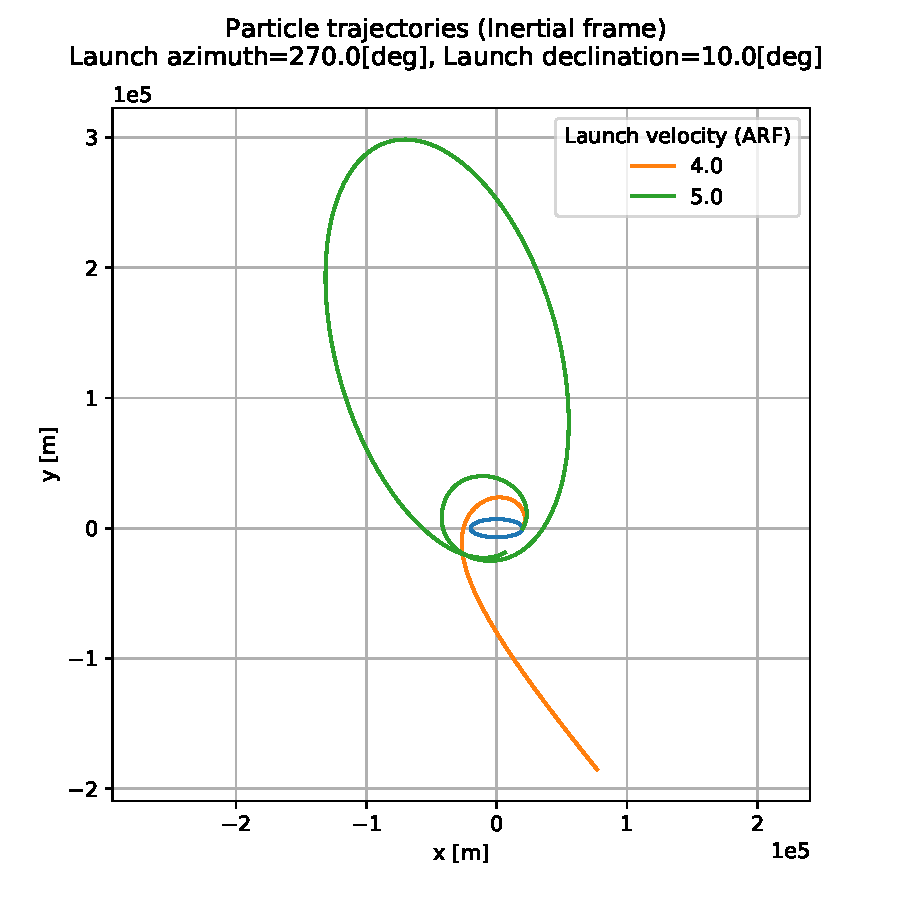
\includegraphics[width=\textwidth, height=0.4\textheight, keepaspectratio=true]{non_conservative_escape_speed/2d_traj_10Decl_4and5_ms.pdf}
    \label{fig:non_conservative_10Decl_4and5_launchVel_2dTraj}
}

\subfloat[]{
    
\includegraphics[width=0.15\textwidth, height=0.15\textheight, keepaspectratio=true]{non_conservative_escape_speed/4ms_10DegDeclination_escape_CDE_qrCode.png}
    \label{fig:non_conservative_10Decl_4ms_animation}
}
\qquad
\subfloat[]{
    
\includegraphics[width=0.15\textwidth, height=0.15\textheight, keepaspectratio=true]{non_conservative_escape_speed/5ms_10DegDeclination_escape_CDE_qrCode.png}
    \label{fig:non_conservative_10Decl_5ms_animation}
}
\caption{Particle trajectories and animation links for the same launch declination of \SI{10}{\degree} but for two different launch velocities, launched from the longest edge of a \gls{CDE} asteroid. \protect\subref{fig:non_conservative_10Decl_4and5_launchVel_2dTraj} shows the equatorial trajectories for the two velocities. To view the trajectory animation for the \SI{4}{\metre\per\second} case, scan the QR code in \protect\subref{fig:non_conservative_10Decl_4ms_animation} or access the web-link \protect\url{https://youtu.be/uulpIO4mbeE}, and for the \SI{5}{\metre\per\second} case, scan the QR code in \protect\subref{fig:non_conservative_10Decl_5ms_animation} or access the web-link \protect\url{https://youtu.be/S9A7oAmmDlg}.}
\label{fig:non_conservative_10Decl_4and5_launchVel}
\end{figure}
\FloatBarrier
%%%

\section{Conservative Approach Limitations With Ellipsoidal Asteroid}
\label{sec:conservative_escape_cde_limitations}
We saw earlier in \Cref{fig:non_conservative_multiple_velocities_qinfinity_0.3} that the \gls{CGES} method was unable to demarcate a few re-impact cases. However, for the same launch location and range of velocities, if the particles are lofted in the normal direction, then the \gls{CGES} method is able to separate out all re-impact cases. This is observed in \Cref{fig:conservative_escape_normal_direction}. Thus, for a situation in which a particle is launched in a direction other than that of the surface normal, with a launch velocity that is above the \gls{CGES}, we observe that the particle does not have to necessarily escape.
%%%
\begin{figure}[htb]
\centering
\captionsetup{justification=centering}
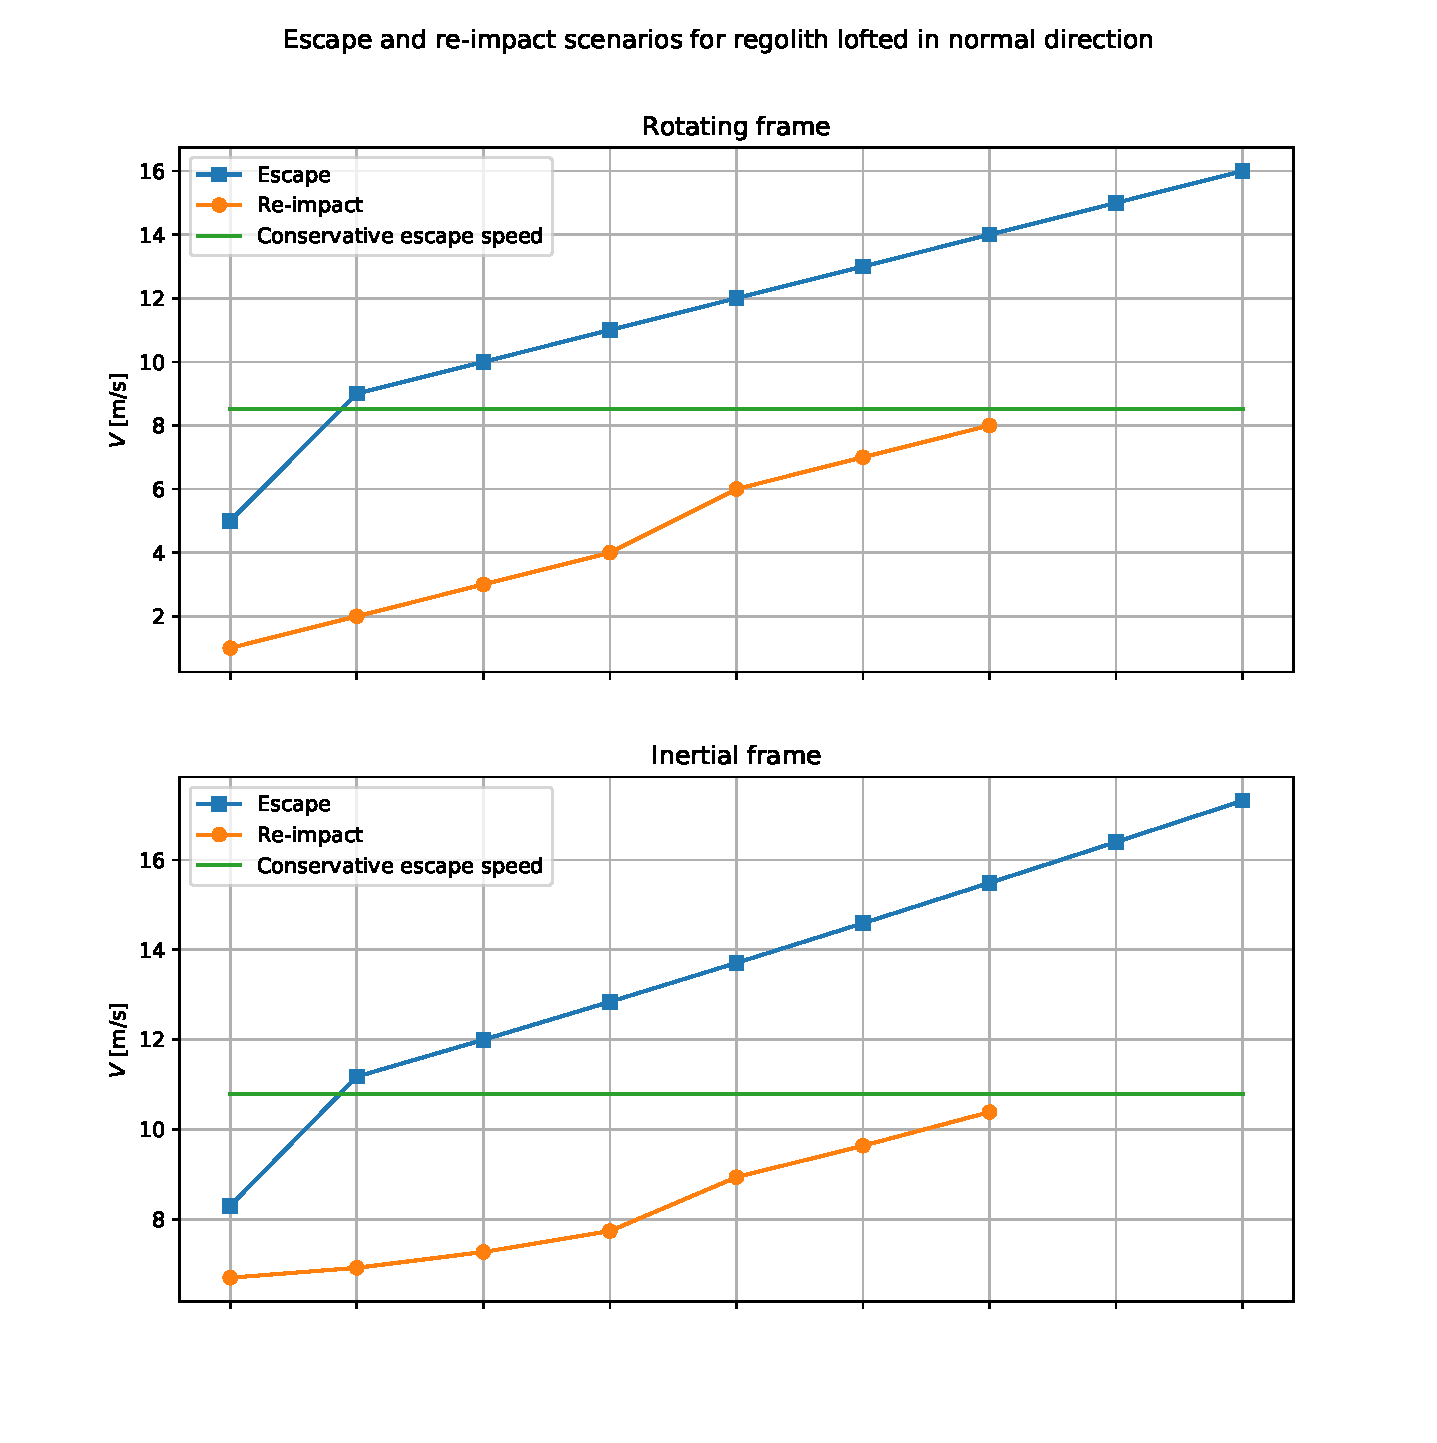
\includegraphics[width=\textwidth, height=0.5\textheight, keepaspectratio=true]{non_conservative_escape_speed/conservative_escape_normal_direction.pdf}
\caption{Escape and re-impact scenarios depicted for regolith launched from the longest edge of \gls{CDE} with multiple velocities and in direction of the surface normal.}
\label{fig:conservative_escape_normal_direction}
\end{figure}
\FloatBarrier
%%%
The \gls{CGES} approach did not account for a few escape scenarios when regolith was launched from the surface of a \gls{CDE}-shaped asteroid and the reason for that is the combined effect of the shape/gravity field variations and a rapid rotation rate of the asteroid. For example, from the trajectory for the regolith launched at a declination angle of \SI{15}{\degree} in \Cref{fig:non_conservative_escape_multiple_qinfinity_single_velocity}, it was observed that the particle completes one revolution around the asteroid before embarking on a final hyperbolic trajectory. This is shown in \Cref{fig:3d_traj_declination_15}.
%
\newline\newline
%
The animation for the trajectory in \Cref{fig:3d_traj_declination_15} can be found at the web-link given in \Cref{fig:declination_15_animation}. The animation clearly shows the rapid rotation rate of the asteroid which accelerates the particle as it approaches behind it and completes the one and only revolution around the asteroid; having its velocity increased enough to eventually attain a positive energy and escape the asteroid. Thus with the help of gravity perturbations and a fast rotating asteroid, the particle changes from an elliptical orbit to a hyperbolic trajectory leading to its escape. This behavior can not be easily captured just from the initial conditions, as we observed, by the \gls{CGES} algorithm.
%
\newline\newline
%
An important thing to note here is that in case of the ellipsoidal asteroid, the particle orbit is osculating because of the non-uniform gravity field. So for a particle that escapes, it is not necessary for it to embark on the escape trajectory immediately after launch. On the other hand, when we consider a spherical asteroid, the launched particle continues to propagate on the initial trajectory itself, because in the absence of perturbations, the initial orbital elements do not osculate. Thus for a spherical asteroid, a particle can only escape if the initial orbit itself is parabolic or hyperbolic. This is why the \gls{CGES} algorithm worked for the spherical asteroid in predetermination of escape situations as we saw in \Cref{fig:conservative_spherical_asteroid_escape}.
%%%
\begin{figure}[htb]
\centering
\captionsetup{justification=centering}
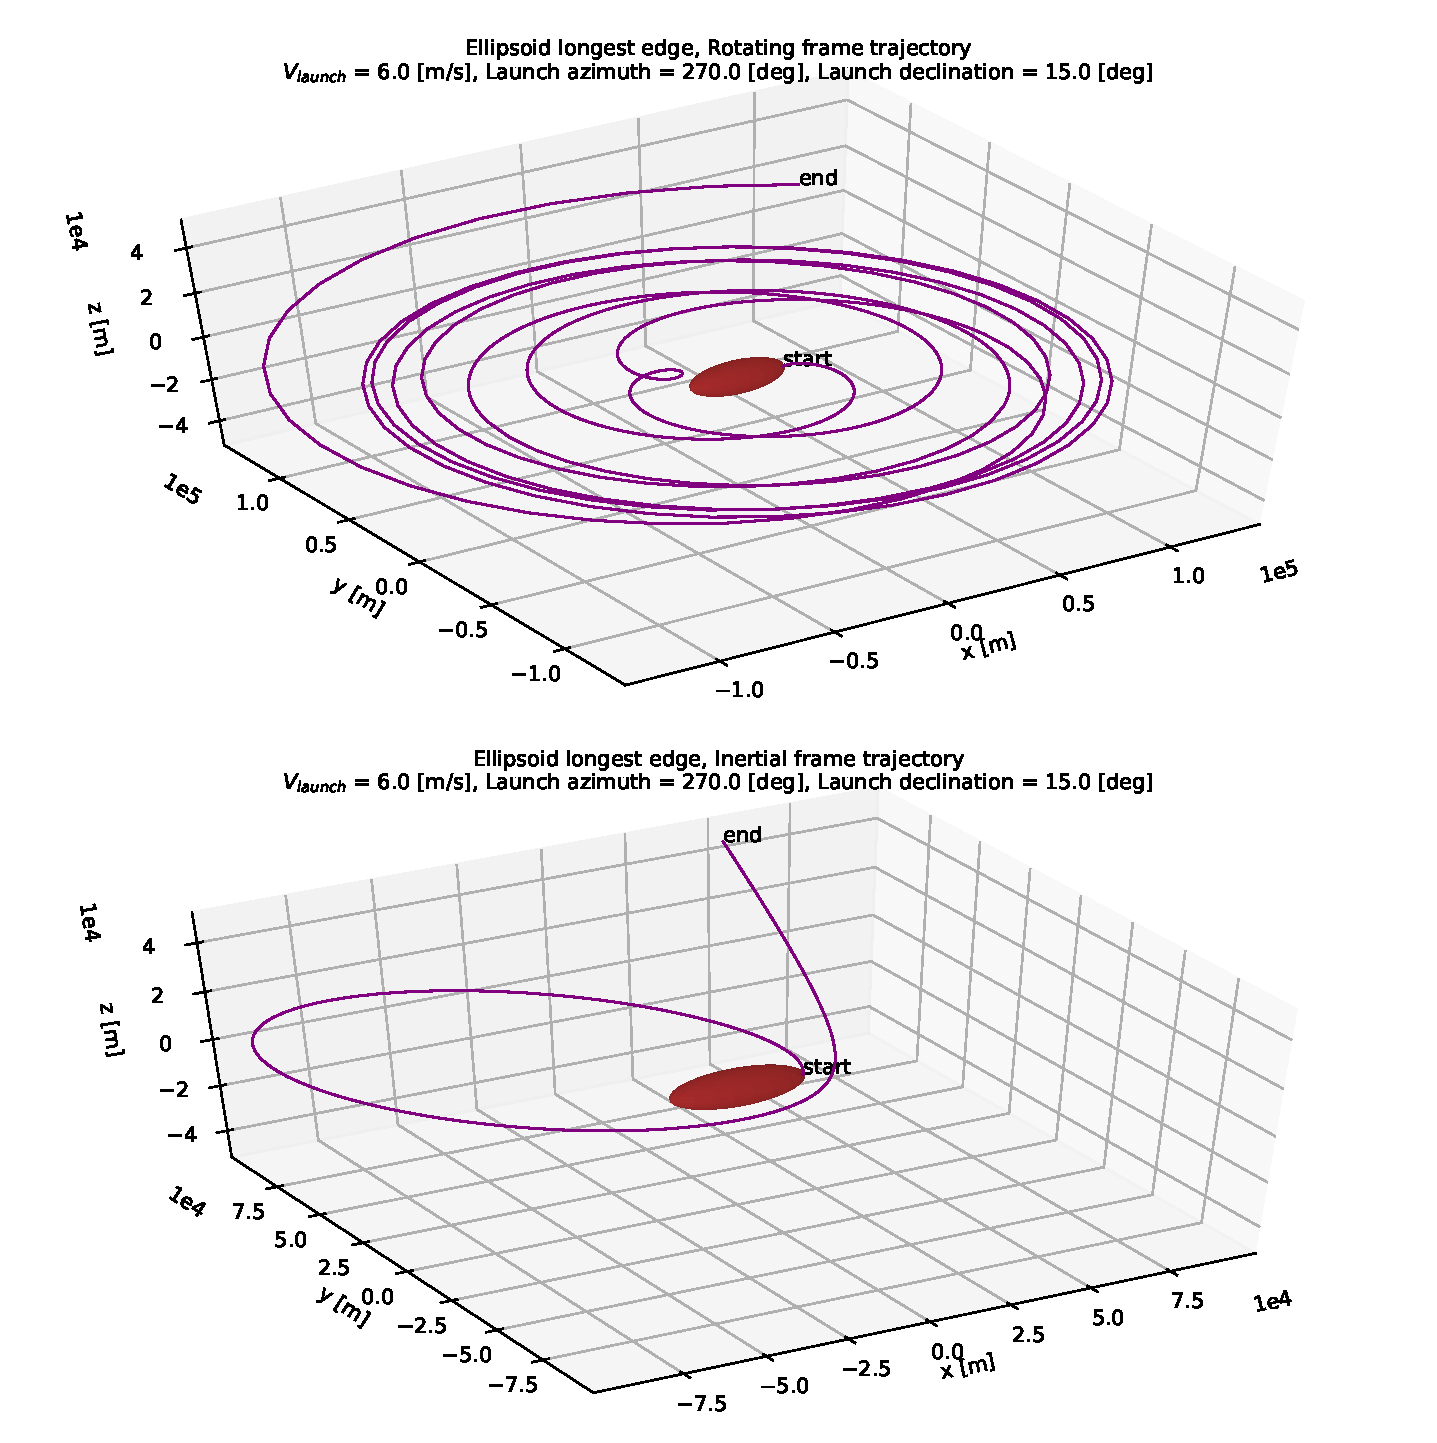
\includegraphics[width=\textwidth, height=0.5\textheight, keepaspectratio=true]{non_conservative_escape_speed/multiRev_3D_trajectory_declination15.pdf}
\caption{3D trajectory in the \gls{ARF} and the \gls{AIF} for launch declination angle \SI{15}{\degree} from \Cref{fig:non_conservative_escape_multiple_qinfinity_single_velocity}.}
\label{fig:3d_traj_declination_15}
\end{figure}
\FloatBarrier
%%%
%%%
\begin{figure}[htb]
\centering
\captionsetup{justification=centering}

\includegraphics[width=\textwidth, height=0.1\textheight, keepaspectratio=true]{non_conservative_escape_speed/declination_15_animation.png}
\caption{Scan the QR code to view the 2D trajectory animation in the \gls{AIF} for launch declination angle \SI{15}{\degree} from \Cref{fig:non_conservative_escape_multiple_qinfinity_single_velocity}. The video can also be accessed from the following web-link: \url{https://youtu.be/5l_CAYnjotk}.}
\label{fig:declination_15_animation}
\end{figure}
\FloatBarrier
%%%
%%%
\begin{figure}[htb]
\centering
\captionsetup{justification=centering}
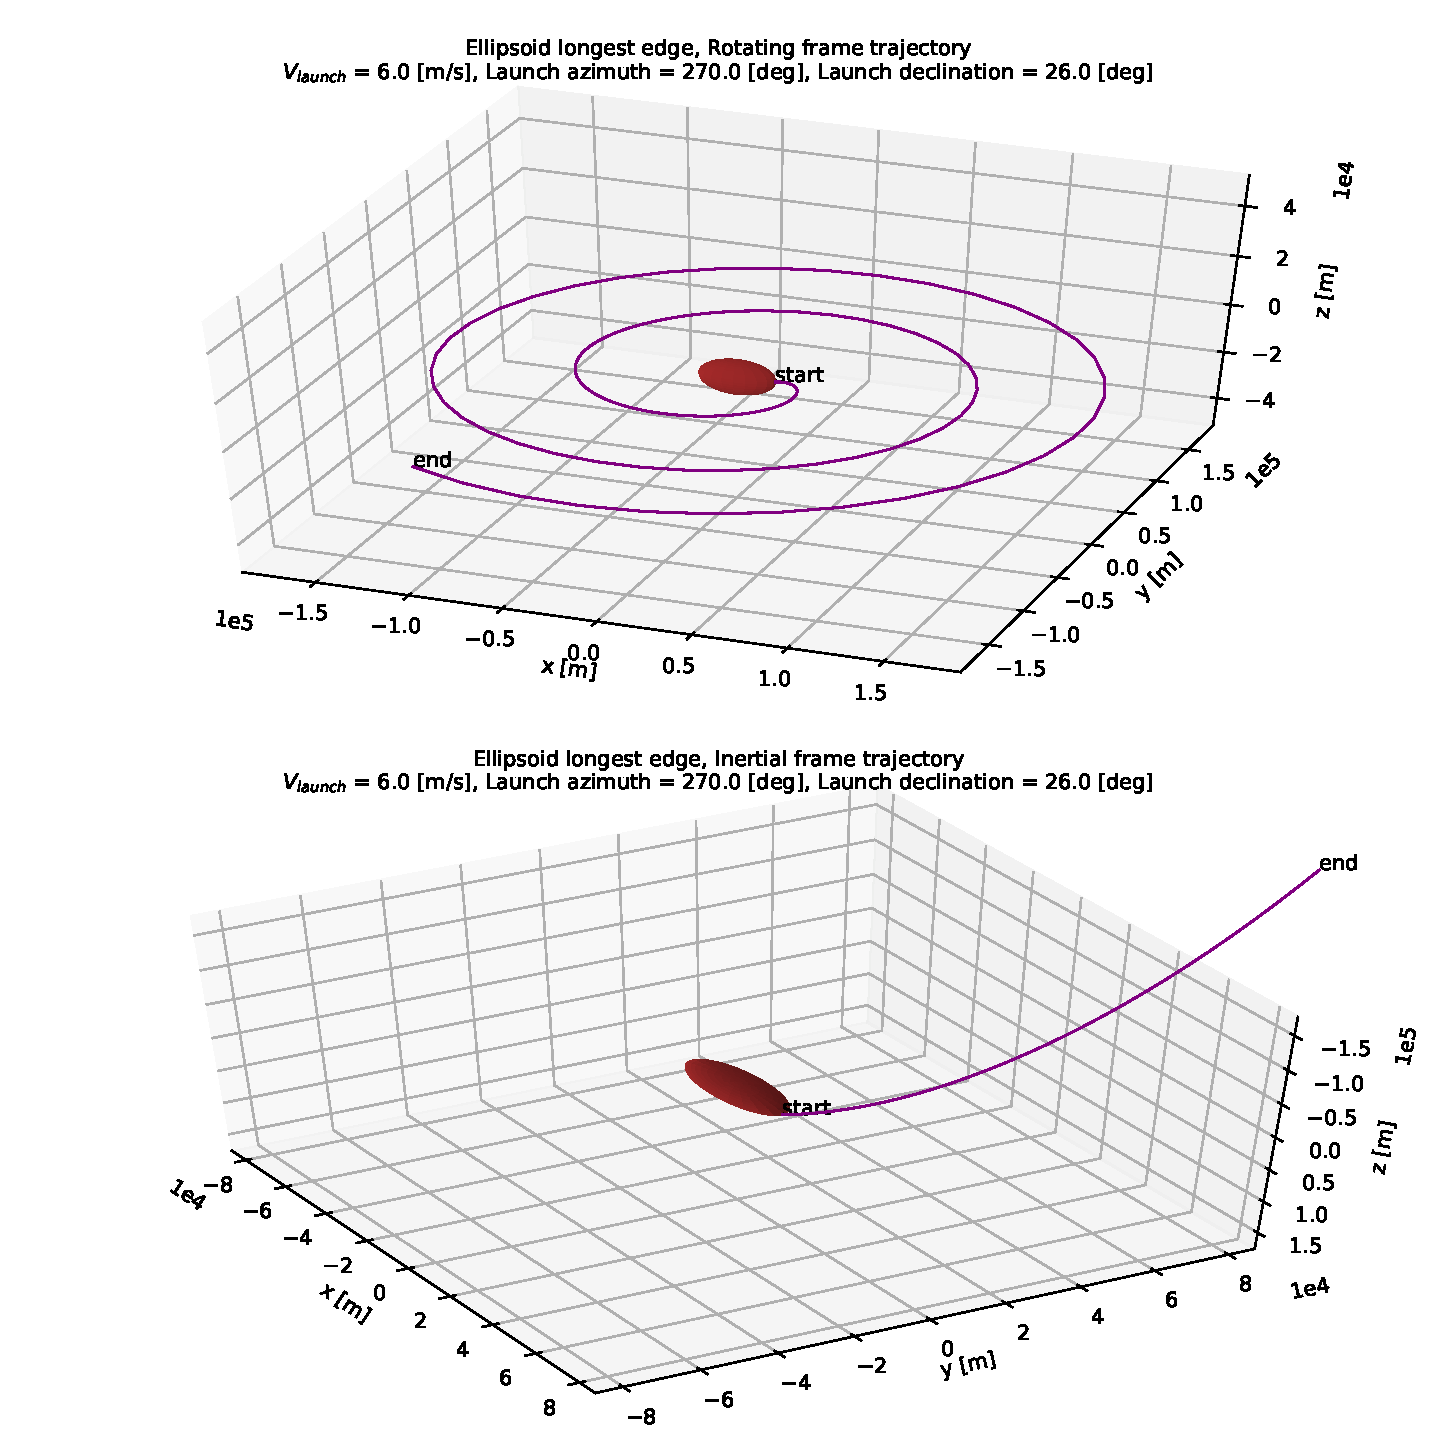
\includegraphics[width=\textwidth, height=0.55\textheight, keepaspectratio=true]{non_conservative_escape_speed/directEscape_3D_trajectory_declination26.pdf}
\caption{3D trajectory expressed in the \gls{ARF} and the \gls{AIF} for a launch declination angle of \SI{26}{\degree} from the normal direction. The particle launch conditions are the same as that used for \protect\Cref{fig:non_conservative_escape_multiple_qinfinity_single_velocity}.}
\label{fig:3d_traj_declination_26}
\end{figure}
\FloatBarrier
%%%
The final aspect that will be discussed in regard to the \gls{CGES} algorithm is its capacity to distinguish between particles that escape immediately and the ones that take one or more revolutions before escaping, when launched from an irregular body \parencite{scheeres2002fate}. However, we found out that this is only true if the particle is launched from the surface in the normal direction. In that, if the launch speed is lower than the \gls{CGES} and the particle escapes, then it underwent multiple revolutions. This was observed for multiple particles launched from the longest edge of the \gls{CDE} for launch velocities ranging from 1 to \SI{16}{\metre \per \second}. However, this phenomenon is not observed when the launch direction is not in the normal direction. For example, from \Cref{fig:non_conservative_escape_multiple_qinfinity_single_velocity}, the launch declination angle of \SI{26}{\degree} results in a direct escape scenario, even though the launch velocity is below the \gls{CGES} curve. The 3D trajectory for this case is shown in \Cref{fig:3d_traj_declination_26}.
%
\newline\newline
%
Thus, it is imperative to understand that with just a non-uniform gravity field and a relatively fast rotating asteroid, the dynamics for orbiting regolith become intangible enough such that predetermination of orbital behavior and final fate of the regolith can not be explained by simple analytical methods. We attempted to explain the complex behavior by deriving a different guaranteed escape speed algorithm, the \gls{NCGES}, however the method failed completely. We realize now that a numerical simulation method is a relatively better approach to understand the orbital dynamics of regolith lofted from an asteroid.

